% =========================================================================
% KSTAR CES 10 ms 결측 채움 -- 8쪽 CVPR 형식 논문(국문, 유일한 논문 판).
% Numbers traced to THESIS_RESULTS.md §0 and the sections it cites (2026-11-11),
% plus the review-loop round-1 analyses (2026-11-13): A1 V_rot fit-failure rule
% (docs/paper/vrot_failfit_sensitivity.json), A2 decomposition
% (docs/paper/b28_decomposition.json), A3 noise-corrected coupling bound
% (docs/paper/fast_target_coupling_bound.json).
% 영문 main_short.tex 의 국문 대응본이며 수치는 같다. 기록 본문에 없는 분할별 값의 출처:
% docs/paper/paper_numbers.json, docs/paper/b27_kfold_interval_R10.json,
% docs/paper/b27c_hier.json, docs/b28_weight_physics_report.md.
% 조판은 preamble_ko.tex 의 LuaLaTeX + luatexko, 함초롬바탕을 따르되,
% 판형은 main_short.tex 의 2단 CVPR 형식을 유지한다.
% 빌드(이 폴더에서): latexmk -lualatex main_short_ko
% =========================================================================
\documentclass[10pt,twocolumn,letterpaper]{article}

\usepackage[textwidth=6.875in,textheight=8.875in,columnsep=0.3125in,
            top=1in,headheight=0pt,headsep=0pt,centering]{geometry}
\usepackage{amsmath,bm}
\usepackage{newtxmath}
\usepackage{luatexko}
\usepackage{graphicx}
\usepackage{booktabs}
\usepackage{multirow}
\usepackage{microtype}
\usepackage[compact]{titlesec}
\usepackage[numbers,sort&compress]{natbib}
\usepackage[colorlinks=true,linkcolor=blue,citecolor=blue,urlcolor=blue,unicode]{hyperref}

% ── 폰트(preamble_ko.tex 와 같은 한글 서체) ──────────────────
\directlua{
  luaotfload.add_fallback("symfallback", {
    "HCR Batang:mode=node;",
    "DejaVu Sans:mode=node;",
    "Segoe UI Symbol:mode=node;",
    "Malgun Gothic:mode=node;",
  })
}
\setmainfont{TeX Gyre TermesX}[RawFeature={fallback=symfallback}]
\setsansfont{Latin Modern Sans}[RawFeature={fallback=symfallback}]
\setmonofont{Consolas}[Scale=0.92]
\setmainhangulfont{HCR Batang}[BoldFont={HCR Batang Bold},AutoFakeSlant=0.2,Scale=0.96]
\setsanshangulfont{HCR Dotum}[BoldFont={HCR Dotum Bold},AutoFakeSlant=0.2,Scale=0.96]
\setmonohangulfont{GulimChe}[AutoFakeBold=1.5,AutoFakeSlant=0.2,Scale=1.0116]

\linespread{1.10}
\setlength{\emergencystretch}{2em}
\registerbreakableafter{"00B7}

\titleformat{\section}{\normalfont\large\bfseries}{\thesection.}{0.5em}{}
\titleformat{\subsection}{\normalfont\normalsize\bfseries}{\thesubsection.}{0.5em}{}
\titlespacing*{\section}{0pt}{8pt plus 2pt minus 2pt}{4pt plus 1pt}
\titlespacing*{\subsection}{0pt}{6pt plus 2pt minus 1pt}{3pt plus 1pt}
\renewcommand{\bibfont}{\small}
\setlength{\bibsep}{1pt plus 0.5pt}
\setlength{\abovecaptionskip}{4pt}
\setlength{\belowcaptionskip}{0pt}
\setlength{\textfloatsep}{8pt plus 2pt minus 2pt}
\setlength{\floatsep}{6pt plus 2pt minus 2pt}
\setlength{\dbltextfloatsep}{8pt plus 2pt minus 2pt}

\renewcommand{\abstractname}{초록}
\renewcommand{\refname}{참고문헌}
\renewcommand{\figurename}{그림}
\renewcommand{\tablename}{표}

\newcommand{\Ti}{\ensuremath{T_i}}
\newcommand{\Vrot}{\ensuremath{V_\mathrm{rot}}}
\newcommand{\skillp}{\ensuremath{\mathrm{skill}_{\mathrm{PCHIP}}}}
\newcommand{\seqv}{\texttt{seq\_v2}}

\graphicspath{{../figures/}}


\hypersetup{
  pdftitle={KSTAR 10 ms 전하교환분광 결측 채움: 같은 위치 고속 진단에서 읽는 이온온도, 자기 이력에서 읽는 회전, 20-parameter 대리 필터},
  pdfauthor={이승상 (Seungsang Lee)},
}

\title{\vspace{-0.3in}\large\textbf{KSTAR 10\,ms 전하교환분광 결측 채움:
같은 위치 고속 진단에서 읽는 이온온도, 자기 이력에서 읽는 회전,
그리고 20-parameter 대리 필터}}
\author{이승상 (Seungsang Lee)\\
  {\small 서울대학교 원자핵공학과}\quad
  {\small\texttt{lss010330@snu.ac.kr}}}
\date{\vspace{-0.25in}}

\begin{document}
\maketitle

% =========================================================================
\begin{abstract}
전하교환분광(CES)은 KSTAR의 이온온도 \Ti{}와 토로이달 회전 \Vrot{}을 한 채널($R =
2.198$\,m)에서 준다. 2022년 캠페인 방전 641개의 10\,ms 격자에서 \Ti{} 표본의 8.2\%,
\Vrot{} 표본의 23.9\%가 결측이다. 우리는 다음 CES 측정 없이 한 스텝을 채워야 할 때, 그
채널에서 1.5\,cm 안에 있는 빔방출분광(BES)과 전자사이클로트론방출영상(ECEI) 채널이 과거
CES에 무엇을 더하는지 묻는다. 2분기 LSTM은 \Ti{}에 대해 고속 채널(각 방전 자신의 통계로
표준화하며, 이는 오프라인 단계다)과 과거 CES를 읽고, \Vrot{}에 대해서는 과거 CES만 읽는다.
\Ti{}의 평균 제곱 오차 skill은 과거 CES의 인과 가우시안 과정 평활기 대비 $+0.113$
$[+0.085, +0.132]$(95\% 구간, 방전 639개의 재분할 8벌)이고, PCHIP 보간 대비 $+0.221$
$[+0.188, +0.248]$인데 그 절반가량은 과거 CES의 1-parameter 이동 평균이 이미 준다. 오프라인
가우시안 과정 대비로는 $-0.010$ $[-0.043, +0.014]$이다. 고속 채널은 동시각 100\,ms 고역 통과
응답으로 들어오며, 그 위에 세운 20-parameter 대리 필터는 PCHIP 대비 skill의 72--78\%를
유지한다. 이득은 꼬리에 있다. 중앙값 절대오차(47.2\,eV)는 persistence의 값(46.1\,eV)에 가깝다. \Vrot{}에서는 고속
채널 증분과 \Vrot{} 증분의 잡음 보정 상관이 10--200\,ms의 모든 시차와 윈도에서
$|r| \leq 0.044$로 묶인다(\Ti{}: $\geq +0.13$). 피팅 실패에 앵커된 0.05\%의 행을 빼면 이력만
쓰는 추정의 skill은 persistence 대비 $+0.265$ $[+0.198, +0.326]$, 인과 평활기 대비 $+0.151$
$[+0.038, +0.290]$이며, 등록된 PCHIP 대비 skill은 그 행들이 실어 나른다. 한 장치, 한 캠페인,
한 채널의 결과다.
\end{abstract}

% =========================================================================
\section{서론}
\label{sec:intro}

이온온도 \Ti{}와 토로이달 회전 \Vrot{}은 페데스탈 구조, ELM 거동, 고성능 운전 영역
접근을 지배한다. 두 물리량은 전하교환분광(CES)~\citep{Ko2010ChargeExchange}으로
측정되며, CES는 전하교환 선의 도플러 확장에서 \Ti{}를, 도플러 이동에서 \Vrot{}을
추정한다. CES는 광자를 적분해야 하므로 느리고 간헐적으로 결측된다. KSTAR 10\,ms
격자에서 \Ti{} 관측의 8.2\%, \Vrot{} 관측의 23.9\%가 서로 독립적으로 결측되고,
\Vrot{} 행의 41.1\%는 여기에 더해 직전 값을 비트 단위로 반복하므로 독립적인 \Vrot{}
측정을 담은 격자는 35.0\%뿐이다. 결측률은 인접 스텝 변화의 오분위를 따라 0.77\%에서
4.45\%로 오르고, BES 세기 최하위 오분위에서 19.9\%, 최상위 오분위에서 3.7\%다. 즉
무작위적이지 않은 결측(MNAR)이다~\citep{Little2002StatisticalAnalysis}. 한편
빔방출분광(BES), 전자사이클로트론방출영상(ECEI), Mirnov 코일은 같은 플라즈마를 결측 없이
보지만, 어느 것도 \Ti{}나 \Vrot{}을 측정하지 않는다. 본 논문의 질문은 이것이다.
\emph{CES가 결측된 10\,ms 시점에서, 동시각 고속 진단은 불규칙한 과거 CES에 무엇을
더하는가?} 쓰임새는 다음 CES 노출을 기다릴 수 없는 추정이다. 양쪽 이웃을 읽는 오프라인 잡음 인지
평활기 대비로는 skill 구간이 0을 포함한다(\S\ref{sec:res:headline}).

\paragraph{비교 대상.}
배치 가능한 비교 대상은 과거 CES만 읽는다. persistence, 이동 평균, 과거 CES 값 16개 위의
인과 가우시안 과정(GP)이다. 선형 보간, PCHIP~\citep{fritsch1980} 보간, 오프라인 GP는 양쪽
이웃을 읽으며 오프라인 참조로 쓴다. PCHIP은 잡음 낀 앵커를 정확히 지나므로, 과거 CES만 쓰는
평활기도 이미 PCHIP 대비 이득을 얻는다(이동 평균의 PCHIP 대비 $+0.05\sim+0.17$, 컷, 3/4
분할에서 구간이 0 제외). 따라서 고속 진단의 기여를 가르는 비교는 인과 GP다.

모든 결과는 두 공동 1차 모집단에서 보고한다. \emph{컷}은 3\,keV를 넘는 \Ti{} 행
0.53\%(스펙트럼 피팅 실패)를 모든 팔에서 결측으로 처리하고, \emph{포함}은 그대로
둔다(\S\ref{sec:data}). 포함 모집단의 추가 여유는 대부분 스파이크 처리에서 온다.

\paragraph{주장.}
\emph{(1) 이온온도.} 같은 위치의 BES와 ECEI는 과거 CES에 동시각 과도 신호를 더한다. 인과
GP 대비 skill은 $+0.113$ $[+0.085, +0.132]$(컷), $+0.118$ $[+0.076, +0.157]$(포함)이고,
20-parameter 대리 필터는 PCHIP 대비 skill의 72--78\%를 유지한다(컷. 그 형태는 사후에
골랐다).
\emph{(2) 회전.} 같은 채널과 \Vrot{} 증분의 잡음 보정 상관은 10--200\,ms에서
$|r| \leq 0.044$로 묶이며, 그 채널이 \Vrot{}에 닿게 하면 4/4 분할에서 skill을 잃는다. \Vrot{}은 자기 이력에서
추정하고(persistence 대비 skill $+0.265$ $[+0.198, +0.326]$, 컷, 피팅 실패 행 제외), 그
10\,ms 산포는 가우스 선 맞춤의 잡음 바닥과 맞는다.
평가(두 공동 1차 모집단, shot 군집 paired bootstrap, 겹침 보정 반복 교차검증 구간, 두 단계
bootstrap, \S\ref{sec:eval})는 표준 조각을 조립한 것으로, 주장이 아니라 방법으로 기술한다.
코드와 평가 산출물은 공개하며, KSTAR shot 파일은 재배포할 수 없다.

% =========================================================================
\section{관련 연구}
\label{sec:related}

\paragraph{결측 채움과 기준선.} GP 회귀~\citep{rasmussen2006}는 핵융합 프로파일
피팅의 표준 도구로~\citep{chilenski2015,michoski2024}, KSTAR CES \Ti{} 프로파일에도
적용되었다~\citep{Kim2024KineticProfile}. PCHIP~\citep{fritsch1980}은 계단에서 스플라인
진동을 피한다. 점수는 Murphy skill~\citep{murphy1988}이다. persistence 기준은 핵융합
프로파일 예보~\citep{Abbate2025Combining}와 우주기상~\citep{Owens2013Persistence}에
선례가 있다.

\paragraph{신경망 진단 추론.} NN-CES는 빔 변조 없이 KSTAR CES 스펙트럼에서 \Ti{}와
회전을 추출한다~\citep{Lee2026NeuralNetworkbased}. 가장 가까운 선행 연구이며 해당
시점의 측정 스펙트럼을 필요로 한다. \emph{NN-CES는 측정된 시점을 더 잘 읽고, 본 연구는
측정되지 않은 시점을 채운다.} \citet{Lin2024PredictionPlasma}는 EAST에서 X선 결정
분광기를 \Ti{}와 회전으로 사상하는데, 같은 광자 채널의 동시각 사상이다.
RTCAKENN~\citep{Shousha2023MachineLearningbased}은 운동 프로파일을 실시간으로 재구성하며
Thomson/CER 입력의 탈락을 견딘다. 거기서 결측은 강건성 조건이고, 여기서는 타겟 자신의
희소성이 문제다.

\paragraph{교차 진단 재구성.} Diag2Diag는 DIII-D에서 동시각 진단으로 Thomson
$T_e$/$n_e$를 합성하며~\citep{Jalalvand2025MultimodalSuperresolution} 기억 없는 MLP를
쓴다. 관련 연구는 COMPASS에서 Thomson을 조밀화하고~\citep{Imrek2026TemporalSuperresolution},
TCV에서 확장 칼만 필터로 Thomson 간격을 인과적으로 채우며~\citep{Pastore2023ModelBased},
EAST의 $T_e$와 $Z_\mathrm{eff}$를 복원하고~\citep{Wang2025TimeSeries,Jia2026TimeSeries},
HL-3에서 채널을 마스킹한다~\citep{Yang2026FusionmaeSelfsupervised}. 이들의 대상은 전자
채널이나 일반적인 조밀 채널이다. 본 연구는 이 계보를 희소한 이온 채널로, 타겟 자신의
불규칙한 과거를 조건으로 하는 추정으로, 사전등록 기준선에 대한 타겟별 검정으로 확장한다.
우리는 이 결합의 선례를 찾지 못했으며, ``찾지 못함''은 ``없음''이 아니다.

\paragraph{방법의 계보.} 관측 마스크는 GRU-D~\citep{Che2018RecurrentNeural}를 따른다. 겹침
보정 구간은 \citep{Nadeau2003Inference}의 것이고, 반복을 먼저 뽑고 방전을 다시 뽑는
재표집은 계층 bootstrap이며~\citep{Saravanan2020Hierarchical}, 대리 필터의 유지 검정은
\citep{Maheswaranathan2020HowRecurrent}의 고정점 판독을 따른다.

% =========================================================================
\section{데이터와 문제 설정}
\label{sec:data}

10\,ms 격자에 정렬한 KSTAR 방전 파일 641개(shot 30801--32751), 총 247{,}207행을
사용한다. 각 행은 BES~\citep{Nam2012AnalysisEdge} 9채널, ECEI~\citep{Yun2010DevelopmentKstar}
4채널, Mirnov 코일 2채널, 시간, 두 CES 타겟을 담는다. \Ti{}는 행의 8.2\%, \Vrot{}은
23.9\%에서 서로 독립적으로 결측되므로 손실은 타겟별로 마스킹한다(그림~\ref{fig:missing}).
두 CES 타겟은 모두 $R = 2.198$\,m의 2022년 채널이다. BES 9채널과 ECEI 4채널은 그 채널에서
약 1.5\,cm 안에 있고, Mirnov 입력 둘은 한 토로이달 위치에 있는 폴로이달 배열 하나의 두
위치다. 행은 $\geq 0.5$\,s 간극에서 연속 세그먼트로 묶이며, 어떤 팔도 간극을 넘지 않는다.

\paragraph{유지된 \Vrot{} 값.} 관측된 \Vrot{} 값의 54\%는 직전 관측의 비트 단위 반복이다
(최대 1{,}214행 연속, 641개 중 499개 파일). 파일은 그 이유를 기록하지 않는다. \Ti{}와
\Vrot{}의 마스크는 행의 72.8\%에서 일치하므로 두 채널은 따로 후처리된다. \Ti{}의 유지값은
226{,}991행 중 1행이다. 유지값은 타겟, 이력 입력, 정규화 통계, 모든 기준선의 앵커 등
\emph{모든 곳에서} 제거되므로, 어떤 팔도 forward-fill로 공짜 점수를 받지 않는다.

\paragraph{피팅 실패와 두 모집단.} \textbf{\Ti{} 1{,}197행(0.53\%)이 3\,keV를
초과한다}(274개 방전의 951개 런, 런의 85\%는 단일 행). 이는 실패한 스펙트럼 피팅이며
보간 앵커도 오염시킨다. 우리는 \textbf{두 공동 1차 모집단}을 사전등록했다.
\emph{컷}($>$3\,keV를 모든 팔에서 결측 처리)과 \emph{포함}(컷 없음)이며, 주장은 두
모집단 모두에서 성립할 때만 조건 없이 진술한다. 임계값은 2.5--4\,keV에서 결과를 바꾸지
않는다(평균 \Ti{} skill $+0.230$, $+0.232$, 3\,keV에서는 $+0.236$).

\begin{figure}[t]
  \centering
  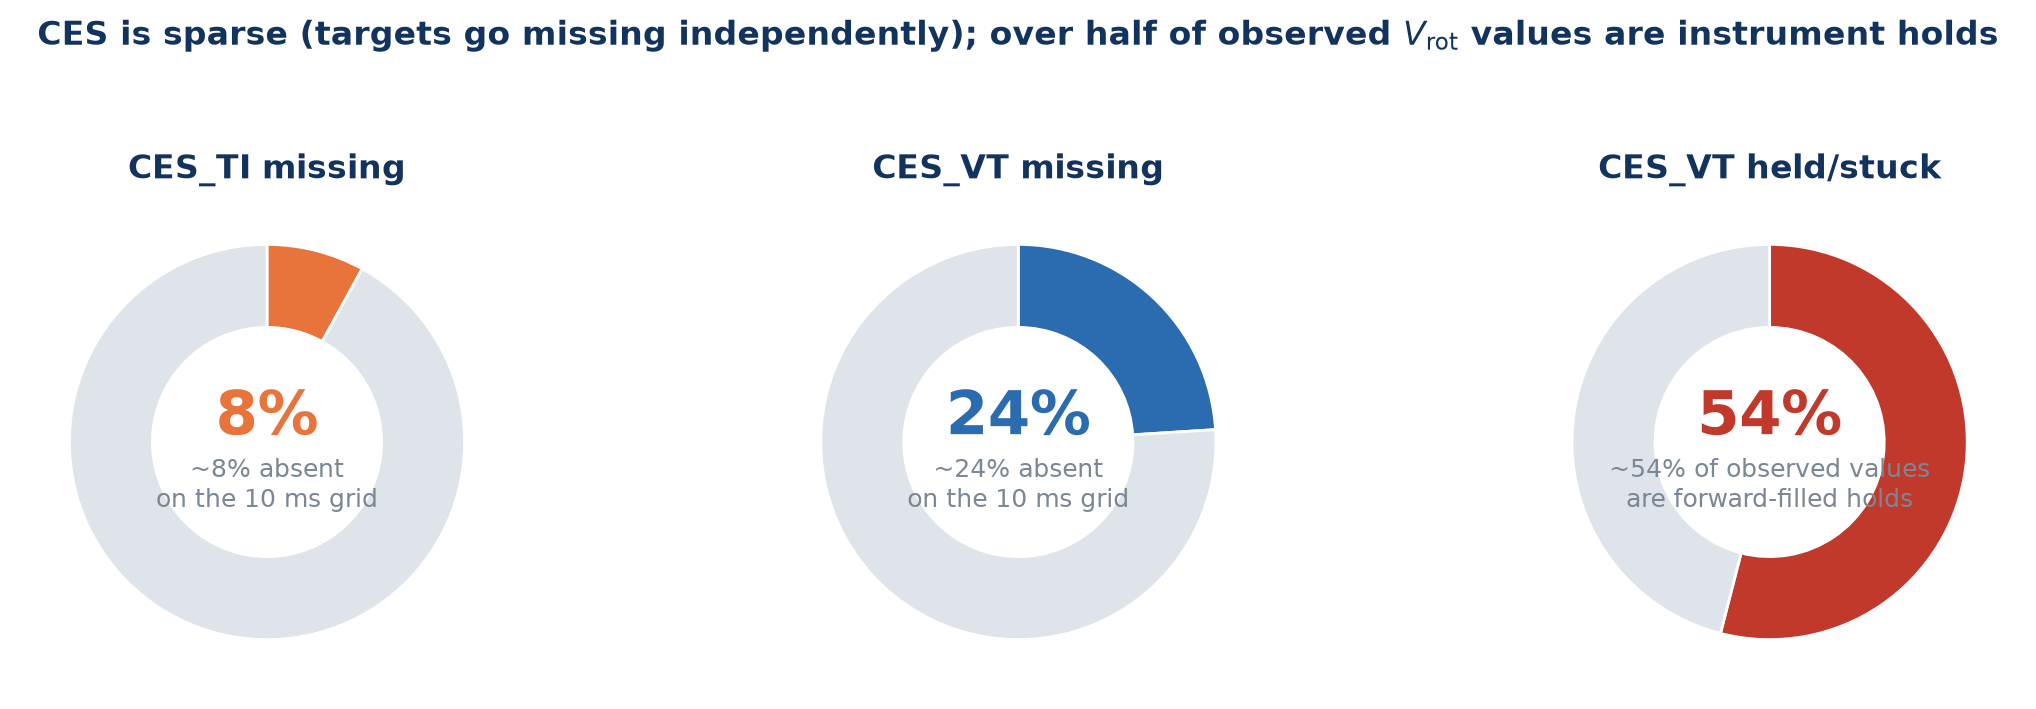
\includegraphics[width=0.92\linewidth]{fig_missing}
  \caption{10\,ms 격자의 CES 결측. \Ti{}와 \Vrot{}은 서로 독립적으로 결측되며(8.2\% /
  23.9\%), 유지값까지 세면 격자의 65.0\%가 독립적인 \Vrot{} 정보를 갖지 않는다.}
  \label{fig:missing}
\end{figure}

% =========================================================================
\section{모델}
\label{sec:model}

주 모델 \seqv{}는 357{,}570 파라미터의 시퀀스 나우캐스터다. 이 절은 무엇을 추정하는지,
왜 입력이 각 타겟에 그렇게 배선되는지, 모델이 어떤 시간 척도 위에 놓이는지, 그리고 그
\Ti{} 분기의 20-parameter 대리 식을 정한다.

\subsection{추정 대상, 손실, 그리고 환원 불가능한 하한}
\label{sec:model:target}
격자 시각 $t$에서 모델은 정규화 타겟 $y_t=[\Ti,\Vrot]_t$를 $x_{\le t}$와 타겟별 관측
마스크 $m_{t,c}\in\{0,1\}$로부터 추정한다:
\begin{multline}
  \mathcal{L}
  = \frac{\sum_{t,c} m_{t,c}\,(\hat y_{t,c}-y_{t,c})^2}{\sum_{t,c} m_{t,c}}\\
  + \lambda\,\overline{\mathrm{ReLU}(z_0-\hat y_{t,\Ti})},\qquad \lambda = 0.1.
  \label{eq:loss}
\end{multline}
첫 항의 최소화 해는 $\mathbb{E}[y_t\mid x_{\le t}]$이고, 둘째 항은 정규화 영점 $z_0$
아래의 \Ti{} 예측을 억제한다. 한 타겟만 관측된 행도 그 타겟을 감독한다(두 타겟을 모두
요구하는 필터는 라벨 행의 $\approx$28\%를 버린다). 타겟 자체가 잡음
$\sigma_\mathrm{meas}$를 지닌 광자 적분 피팅이므로, 완벽한 물리 추정도
$\mathrm{RMSE}^2=\sigma_\mathrm{meas}^2+b^2$를 기록한다. 차분 estimator로 잰 컷 모집단 \Ti{}의
$\sigma_\mathrm{meas}$는 46.4--129.9\,eV로 백본의 157.8\,eV와 같은 자릿수이고, 4차 차분
제곱질량의 46.6\%(\Vrot{}은 65.6\%)가 상위 1\%의 한 스텝 변화에 있다. 즉
식~\eqref{eq:loss}는 \emph{꼬리 통계}다(\S\ref{sec:res:dual}).

\subsection{두 보존식과 입력 라우팅}
\label{sec:model:physics}
이온 에너지와 토로이달 각운동량은 다음을 따른다.
\begin{align}
  \partial_t\bigl(\tfrac{3}{2}n_i T_i\bigr) + \nabla\!\cdot\!\mathbf{q}_i
    &= Q_{ei}\,(T_e-T_i) + S_i,
  \label{eq:energy}\\
  \partial_t\bigl(n_i m_i \langle R^2\rangle \omega_\varphi\bigr)
    + \nabla\!\cdot\!\Pi_\varphi
    &= T_\mathrm{NBI} + T_\mathrm{NTV} + T_\mathrm{int} + \cdots
  \label{eq:momentum}
\end{align}
두 식 모두 변화율을 구속한다. 식~\eqref{eq:momentum}의 항 가운데 NBI 토크와 NTV 토크는
여기에 채널이 없고(Mirnov $dB/dt$는 정적인 $\delta B$를 볼 수 없다), BES 세기는 운동량 유속
$\langle v_r v_\varphi\rangle$가 아니며, 잔여응력은 $\nabla T_i$를 필요로 한다. 실측으로 고속
채널과 $d\Vrot/dt$의 상관은 $r = -0.006$(BES), $-0.003$(ECEI)이고, $d\Ti/dt$와는 $+0.070$,
$+0.078$이다(값 수준: \Ti{} $+0.341$, $+0.311$, \Vrot{} $+0.027$, $+0.005$). 타겟 잡음을
보정하면 고속 채널 증분과 \Vrot{} 증분의 상관은 모든 시차(0--200\,ms)와 윈도(10--200\,ms)에서
95\% 상한 $|r| \leq 0.044$를 가지며, \Ti{}는 50\,ms 이하 윈도에서 하한 $+0.127$을 가진다.
이는 선형 연관의 상한이지 부재의 증명이 아니다(BES의 100--200\,ms에서 $r \approx +0.01$이고
그 구간은 0을 제외한다). 공유 인코더로 고속 채널이 \Vrot{}에 닿게 한 모델은 네 분할 모두에서
\Vrot{} skill을 잃는다(짝지은 $-0.044$, $-0.072$, $-0.067$, $-0.023$). 그래서 분기를
인코더에서 나눈다. \Ti{}에서 고속 채널 응답은 CES 채널에서 1.5\,cm 안에 있는 채널들의 동시각
공동 움직임이다(\S\ref{sec:model:eq}). 그 기전은 여기서 규명하지 않는다. 방전별 표준화가
충돌 교환에 필요한 $T_e$와 $n_e$의 절댓값을 지우고, 파일에는 빔 파워나 D-alpha 신호가 없기
때문이다.

\subsection{시간 척도}
\label{sec:model:scales}
격자 간격 $\Delta t=10$\,ms에서 $f_\mathrm{Nyq}=1/(2\Delta t)=50$\,Hz다. 모드 회전은 kHz
대역에 있으므로(이 데이터셋의 가장자리 조화 진동은 약 4와 8\,kHz), 반앨리어싱 없이
100\,Hz로 데시메이트한 $dB/dt$는 그것을 담을 수 없다. Mirnov의 lag-1 자기상관
$-0.009$(BES $+0.568$)가 이를 확인한다. 자기상관 $1/e$ 시간은 \Ti{}(159\,ms), BES(161),
ECEI(147)에서 일치하지만, \Vrot{}은 유지값을 빼면 16\,ms, 넣으면 300\,ms를 넘는다.
\Vrot{}의 완화 시간은 이 데이터셋에서 측정할 수 없다.

\subsection{전체격자 시퀀스 백본}
\label{sec:model:backbone}

\begin{figure*}[t]
  \centering
  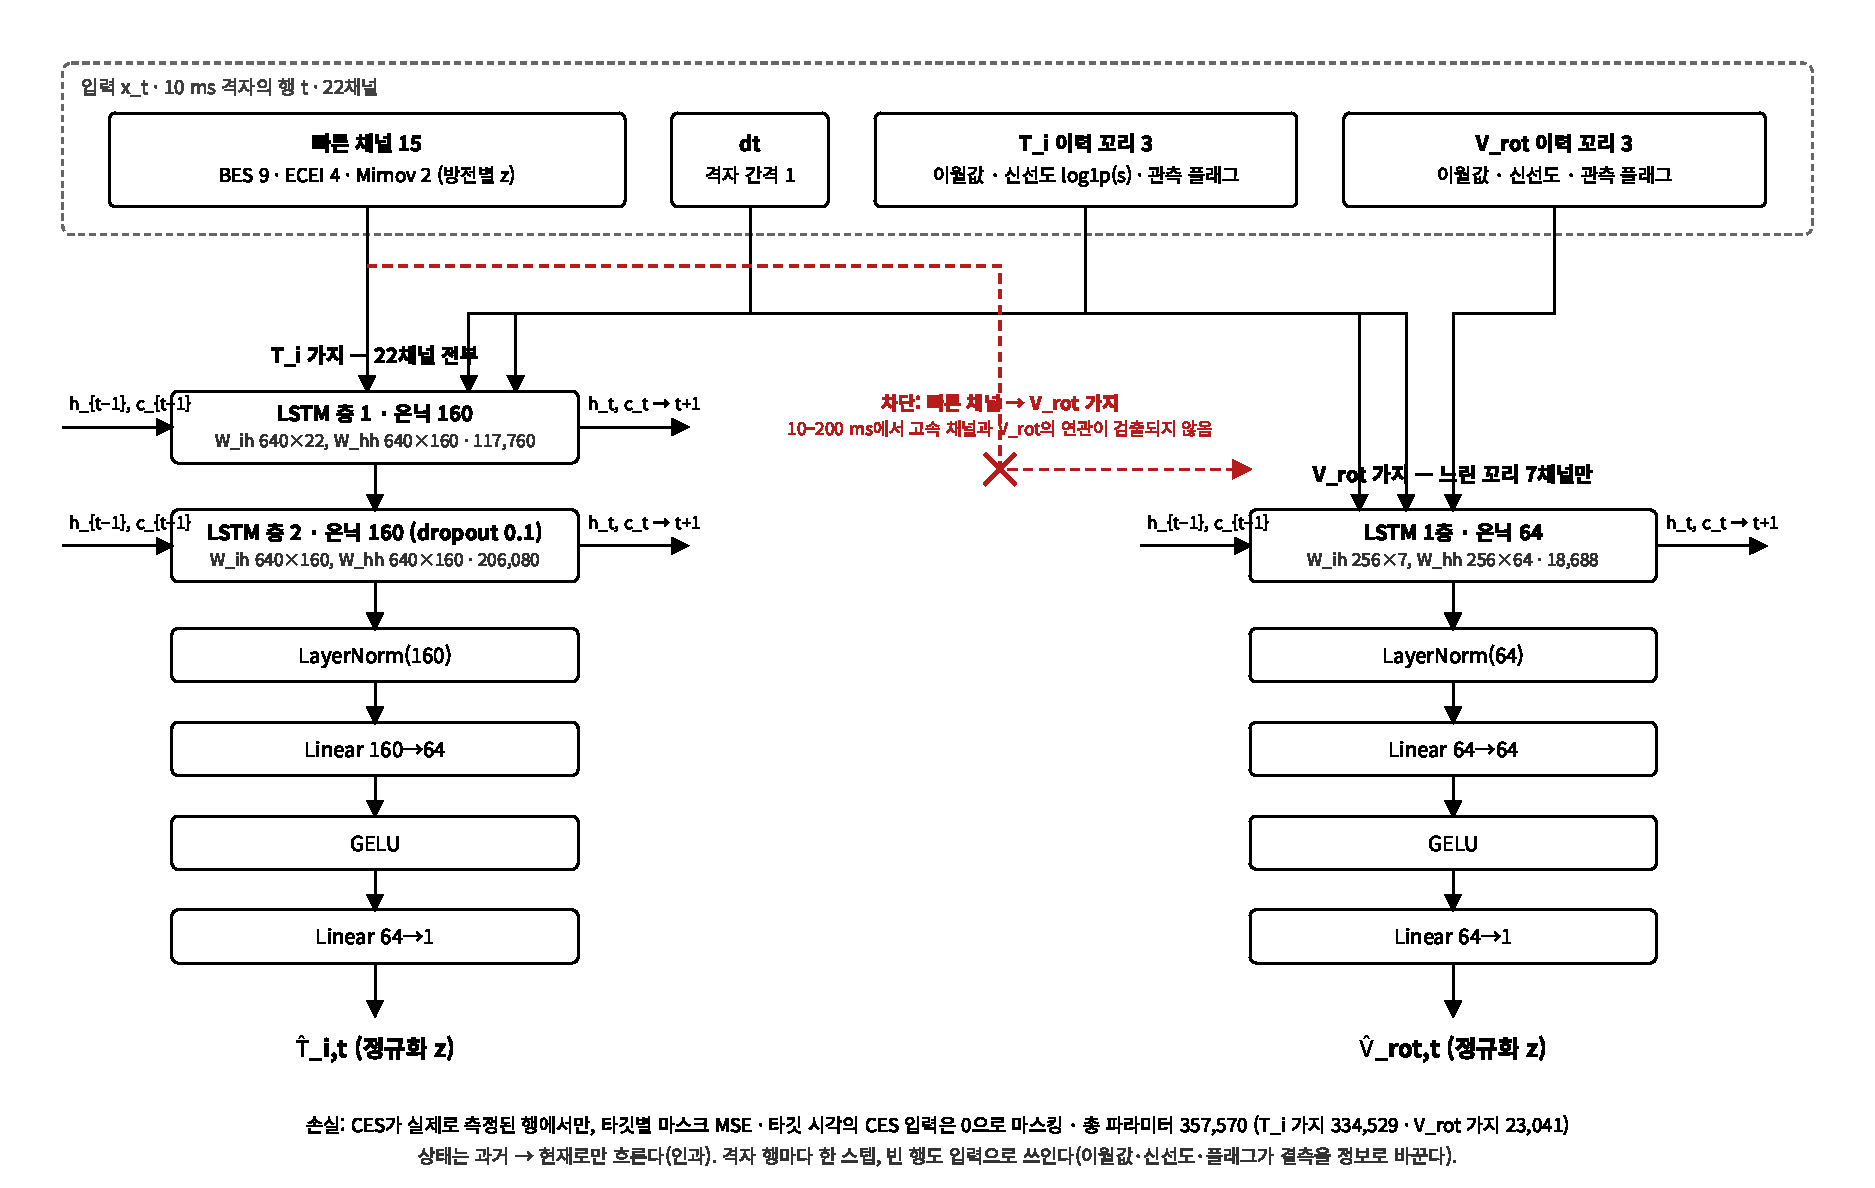
\includegraphics[width=0.8\textwidth]{fig_arch_seq_v2_ko}
  \caption{격자 행 $t$ 하나에 대한 \seqv{}. 입력 22채널(고속 15, 방전별 $z$(방전 전체
  통계); $\Delta t$; 타겟별 이월값, 경과시간, 관측 플래그)이 시간 순방향으로 도는 두 LSTM으로
  들어간다. \Ti{} 분기는 22채널 전부를 읽고(2층, 160 유닛), \Vrot{} 분기는 느린 7채널만
  읽으며(1층, 64 유닛), 각각 LayerNorm과 Linear--GELU--Linear로 끝난다. 고속 채널에서
  \Vrot{}으로 가는 붉은 점선 경로는 구조상 존재하지 않는다. 총 357{,}570 파라미터.}
  \label{fig:arch}
\end{figure*}

고속 진단에는 결측이 없으므로, \seqv{}는 연속 세그먼트의 입력이 완전한 모든 행을 라벨
유무와 무관하게 맥락으로 유지한다(그림~\ref{fig:arch}). 각 스텝은 22개 채널을 담는다.
CES에서 나온 입력은 모두 $t$ 이전 행만 쓰고, 고속 채널 15개는 그 방전 자신의 평균과
분산으로 표준화하는데, 이는 오프라인 단계다. CES에서 나온 채널은
$\log(1{+}\Delta t_\mathrm{prev})$, 그리고 타겟별로 $t$ 이전 행에서 이월된 마지막 관측값,
$\log(1{+}\text{경과시간})$, 과거 관측 존재 플래그다. \Ti{} 분기는 전부를 읽고, \Vrot{}
분기는 고속이 아닌 7개 채널만 읽는다. 이것이 \S\ref{sec:model:physics}의 구현이다. 분기가
인코더에서 나뉘므로 고속 정보를 \Vrot{} 헤드로 나르는 공유 순환 상태는 없다. 출력은 행별
정규화 $[\Ti,\Vrot]$이며, 모든 라벨 행에 대해 식~\eqref{eq:loss}로 학습한다(AdamW,
$\eta=10^{-3}$, weight decay $10^{-4}$, 배치 16 세그먼트, clipping 1.0, 최대 30 epoch의
조기 종료). 분할은 파일 단위이고 다른 모든 채널의 정규화는 학습 파일 전용이며, 타겟 행은
입력에 들어가지 않는다. 이 프로토콜에서 인과(학습 통계) 표준화의 비용은 측정하지 않았다.
피팅 실패 컷이 없던 이전 프로토콜에서 그 변형은 PCHIP 대비 \Ti{} skill $+0.22\sim+0.30$을
유지했고 4/4 분할에서 구간이 0을 제외했다. 백본 자신의 문맥을 자르면 20\,ms에서 $-0.066$을
잃고 50\,ms에서 포화한다. 과거는 이월된 CES 값과 약 50\,ms의 고속 채널 문맥을 통해 \Ti{}
출력에 닿는다.

\paragraph{윈도 대조군과 관문.} 대조군(201{,}258 파라미터)은 방전별 표준화 없이 돌며, 각
모달리티를 직전 $W{=}2$ 행 위의 전용 시간 인지 1-D CNN으로 인코딩하고, CES 이력을 양방향
GRU로 읽은 뒤 타겟마다 하나씩의 멀티헤드 어텐션 readout으로 풀링한다. 어텐션은 하드
마스킹되어 그 타겟이 실제로 측정된 행에만 질량을 둔다. 그 \Vrot{} 헤드도 이력과 시간만
융합한다. 전체격자 프레이밍은 분할 $\times$ 초기화 시드의 $4\times4$ 격자에 대한 사전등록
4조건 관문으로 채택되었다. 짝지은 \Ti{} skill은 16/16 실행에서 양수이고, 합산하면 $+0.081$
$[+0.067, +0.096]$이다. 대조군의 인과 GP 대비 skill은 $+0.041$이다(컷, 3/4 분할에서 구간이
0 포함).

\paragraph{크기와 비용.} persistence에서 출발해 유계 tanh 잠재를 더하는 해석 가능한
칸(21{,}498 파라미터)의 백본 대비 짝지은 \Ti{} skill은 컷에서 $+0.002$(모든 구간이 0
포함)이지만 포함 모집단에서 $-0.194$이므로, LSTM이 백본으로 남는다. 상태 유지 스텝 하나의
비용은 CPU에서 중앙값 0.97\,ms, p99 1.49\,ms이며, 배치에는 인과 표준화가 필요하다.

\subsection{\texorpdfstring{\Ti{} 분기의 20-parameter 대리 식}{Ti 분기의 20-parameter 대리 식}}
\label{sec:model:eq}
동결된 \seqv{} 체크포인트 30벌에 대한 사전등록 판독에서 가중치 크기는 안정된 정보를
주지 않았다(첫 층 열 노름은 고속 채널 15개에서 평평하고, 채널별 순위는 분할 간에
재현되지 않는다). 반면 입출력 응답은 정보를 준다. \Ti{} 출력은 과거 관측 \Ti{}의 지수가중
평균에 고속 채널에 대한 동시각 응답을 더한 것이고, forget 게이트의 기억은 격자 1.3
스텝이다. 판독은 등록된 네 단계로 진행했다.
\emph{(1) 동결 행:} 맞춤 파라미터가 없는 이동 평균 하나가 persistence 대비 백본 skill의
73--82\%(컷)를 내고, 10\,ms 증분 15개에 대한 ridge 선형 항을 더하면 77--85\%가 된다(4/4
분할이 문턱 0.75 이상).
\emph{(2) 학습된 증분 형태:} 같은 식을 처음부터 학습하면 PCHIP 대비 skill의 50--66\%만
유지해 문턱 0.70에 못 미치고, 교차항은 $0.001$ 미만을 더한다.
\emph{(3) 야코비안:} 동결된 TEST 행 전부에서 백본의 고속 채널 응답은
${\approx}100$\,ms 고역 통과(현재값에서 직전 10스텝 평균을 뺀 것)이고, 이득은 $2\sigma$까지
평탄하다가 $3\sigma$ 너머에서 꺼지며 직전 증분에 의존하지 않는다. 3단계는 4단계를 채점하는
같은 네 분할의 TEST 행에서 백본의 야코비안을 읽었으므로, 그 유지는 사후적이다.
\emph{(4) 교정된 형태}를 동일한 프로토콜로 처음부터 학습한다:
\begin{gather}
  \hat y_t = m_t + \sum_{c=1}^{15} a_c\, d_{c,t}\,
     \sigma\!\Bigl(\frac{\theta-|d_{c,t}|}{0.5}\Bigr) + b_0,
  \label{eq:b28h}\\
  d_{c,t} = x_{c,t} - \overline{x}_{c,\,t-10..t-1},
  \nonumber\\
  m_t = m_{t-1} + K(s)\,(y^\mathrm{obs} - m_{t-1}),
  \nonumber\\
  K(s) = K_\infty + (K_0 - K_\infty)\,e^{-s/s_K}.
  \label{eq:gain}
\end{gather}
여기서 $m_t$는 \Ti{} 측정이 새로 들어올 때만 갱신되고, $s$는 직전 측정 이후의 공백이며,
$\sigma(\cdot)$는 로지스틱 함수이고, $d_{c,t}$와 $\theta$는 방전별 표준편차 단위다(오프라인
정규화). 세그먼트의 첫 관측은 그대로 받는다($K=1$). 20개 파라미터는 이득 상수 셋, 고속
채널마다의 이득 $a_c$, 문턱 $\theta$, 오프셋 $b_0$이다. 컷 네 분할에서 학습된 값은 새 측정
직후 $K_0 = 0.27$--$0.30$, 긴 공백 뒤 $K_\infty = 0.48$--$0.53$, 전이 $s_K = 39$--$47$\,ms,
$\theta = 2.9$--$3.0\sigma$, $\sum a_{\mathrm{BES}} = +48\sim+53$,
$\sum a_{\mathrm{ECEI}} = +44\sim+50$\,eV/$\sigma$다. 필터로 읽으면, 기다린 시간이 길수록 새
CES 표본을 더 믿는 칼만형 관측 갱신에, 각 고속 채널의 100\,ms 기준선 대비 편차에 대한 선형
응답을 $3\sigma$ 너머의 이상치에서 차단한 항을 더한 것이다. 이 식의 백본 skill 유지는
\S\ref{sec:res:eq}에 있다. 독립 estimator로서 그 skill(컷)은 PCHIP 대비 $+0.13\sim+0.21$(4/4
분할), 인과 GP 대비 $+0.02\sim+0.07$(2/4에서 구간이 0 제외)이고, 4/4에서 오프라인 GP보다
낮다. 이는 모델에 대한 측정이며, 헤드라인 수치는 여전히 백본의 것이다.

% =========================================================================
\section{평가 방법론}
\label{sec:eval}

\paragraph{지표와 기준선.} 오차는 물리 단위로 타겟별로 계산하며, 1차 점수는
$\skillp = 1 - \mathrm{MSE}_{\mathrm{model}}/\mathrm{MSE}_{\mathrm{PCHIP}}$(0 = 오차가 같음)다.
모든 팔은 동일한 (파일, 행) 집합에서 채점된다. persistence, 이동 평균, 두 점 외삽은 과거만
읽고, 선형·PCHIP·오프라인 GP(Matérn-3/2 + 백색잡음, 최근접 16+16 이웃, 표본별 주변우도
선택)는 미래를 읽는다. 인과 GP는 같은 GP를 과거 이웃 16개로 제한한 것이다. 미래 이웃이 없는
곳에서는 보간이 persistence 값을 예측한다(채점된 \Ti{} 행의 0.2\%, 채점된 \Vrot{} 행의
0.3--0.5\%).

\paragraph{분할과 사전등록.} 파일은 네 시드(42, 1, 7, 123)로 train/val/test에 분할된다.
test 파일은 아키텍처 탐색보다 먼저 예약되었지만, 시퀀스 백본, 방전별 표준화, 대리 식 형태의
채택에는 같은 네 test 분할의 결과를 썼다. 반복 교차검증은 같은 639개 방전을 재분할한다. 표준
test 셋은 96개 shot의 \Ti{} 32{,}589행과 60개 shot의 \Vrot{} 10{,}463행이다(컷).
``사전등록''은 한 배치의 가설, 판정 규칙, 수치 예측을 실행 전에 저장소에 커밋했다는 뜻이며,
제3자 등록소는 없다.

\paragraph{구간.} 표본별 짝지은 제곱오차 차이를 shot 단위로 집계하고 shot 전체를 재표본한다
(10{,}000회). 결과는 95\% 구간이 0을 제외하는지와 함께 보고한다. 분할이 넷뿐이므로 네 값의
평균 $\pm$ 표준편차 대신 분할별 값과 그 구간, 범위, 구간이 0을 제외한 분할 수를
적는다~\citep{Weissgerber2015Beyond,Agarwal2021Deep}. 네 분할은 학습 방전 대부분을
공유하므로, 백본을 639개 방전의 shot 단위 반복 5겹 교차검증으로 다시 돌렸다(반복 10회,
100회 실행, 반복마다 모든 방전을 한 번씩 시험).
\emph{겹 단위}: Nadeau--Bengio 구간
$\bar S \pm t_{0.975,n-1}\sqrt{(1/n + n_{\mathrm{test}}/n_{\mathrm{train}})\,s^2}$~\citep{Nadeau2003Inference}.
\emph{합산}: 한 반복의 test 다섯 겹을 이어 붙여 하나의 skill로 채점하고, 반복 하나를 먼저
뽑은 뒤 그 반복의 방전을 다시 뽑는 두 단계 bootstrap을 쓴다. 반복 교차검증은 겹 단위 구간을
판정 판독으로 등록했으며, \Vrot{}의 PCHIP 대비 구간은 0을 포함했다. 그 뒤 합산 판독을 사후에
계산했고, 새 반복 8회를 실행하기 전에 합산 두 단계 판독을 판정 기준으로 하여 등록했다. 이
구간은 학습된 모델을 조건으로 하며 겹치는 학습 집합 사이의 상관을 담지 않는다. 겹 단위 구간은
그것을 담는다.

% =========================================================================
\section{결과}
\label{sec:results}

\subsection{RMSE 사다리}
\label{sec:res:ladder}
표~\ref{tab:ladder}는 표준 test 분할의 물리 단위 RMSE다. 미래를 읽지 않는 방법 가운데
\seqv{}의 RMSE가 가장 낮아 인과 GP보다 4\%(\Ti)와 18\%(\Vrot) 낮고, 선형·PCHIP 보간보다도
낮다. 잡음 낀 앵커를 평균하는 오프라인 GP가 \Ti{} RMSE가 더 낮은 유일한 팔이다(153.8 대
157.8). 이 데이터에서 더 강한 오프라인 보간은 선형 보간이다. 분할별 \Ti{}의 선형 보간 대비
skill은 $+0.136\sim+0.226$(컷), $+0.209\sim+0.288$(포함)로 두 모집단 모두 4/4 분할에서
구간이 0을 제외하며, PCHIP 대비 skill보다 0.01--0.05 낮다. \Vrot{}에서는 각 모집단 1/4
분할에서 구간이 0을 제외한다.

\begin{table}[t]
  \centering
  \caption{RMSE. 시드 42 test 분할, 컷 모집단, 진짜 측정만($n = 32{,}589$ \Ti{},
  $10{,}463$ \Vrot{}). 아래쪽 행은 미래를 읽는다. 포함 모집단: \seqv{} 363.0 / 23.7,
  PCHIP 412.4 / 30.2, 인과 GP 394.6 / 28.8, persistence 478.0 / 33.4.}
  \label{tab:ladder}
  \footnotesize
  \setlength{\tabcolsep}{3pt}
  \begin{tabular}{llrr}
    \toprule
    팔 & 정보 & \Ti{} (eV) & \Vrot{} (km/s) \\
    \midrule
    \textbf{\seqv{}} & 고속 + 과거 CES, 세그먼트 & \textbf{157.8} & \textbf{23.6} \\
    20-param. 대리 식 & 고속 + 과거 CES & 162.3 & -- \\
    윈도 대조군 & 고속 + 과거 CES 2행 & 169.2 & 26.1 \\
    인과 GP & 과거 CES 16개 & 164.3 & 28.8 \\
    이동 평균 & 과거 CES & 169.2 & -- \\
    Persistence & 마지막 관측 CES & 197.2 & 33.4 \\
    두 점 외삽 & 과거 CES 2개 & 472.2 & 51.0 \\
    \midrule
    GP (오프라인) & 과거 + 미래 CES & 153.8 & 24.7 \\
    선형 보간 & 과거 + 미래 CES & 169.8 & 29.0 \\
    PCHIP & 과거 + 미래 CES & 173.6 & 30.2 \\
    \bottomrule
  \end{tabular}
\end{table}

\subsection{헤드라인과 재현}
\label{sec:res:headline}

\begin{table*}[t]
  \centering
  \caption{비교 대상별 \seqv{}의 skill. \emph{네 분할}: 시드 42/1/7/123에 걸친 분할별
  skill의 범위와, shot 군집 95\% CI가 0을 제외하는 분할 수. \emph{겹 단위}: 반복 5겹
  CV의 50겹에 대한 Nadeau--Bengio 95\% 구간과, 자체 CI가 0을 제외하는 겹 수. 처음 등록할
  때의 판정 판독이다. \emph{합산}: 같은 639개 방전의 재분할 8벌에 대한 중앙값과 두 단계
  bootstrap 95\% 구간으로, 그 반복들을 실행하기 전에 판정 기준으로 등록했다. 굵은 글씨 =
  구간이 0을 제외. 네 분할의 오프라인 GP 칸은 두 모집단을 합친 것이다. \Vrot{} 행은
  \S\ref{sec:res:headline}의 피팅 실패 규칙을 적용하지 않은 등록 판독이다.}
  \label{tab:headline}
  \footnotesize
  \setlength{\tabcolsep}{3pt}
  \resizebox{\textwidth}{!}{%
  \begin{tabular}{llcccccc}
    \toprule
    & & \multicolumn{2}{c}{네 분할} & \multicolumn{2}{c}{겹 단위 (반복 5겹)} & \multicolumn{2}{c}{합산 (두 단계)} \\
    \cmidrule(lr){3-4}\cmidrule(lr){5-6}\cmidrule(lr){7-8}
    타겟 & 대비 & 컷 & 포함 & 컷 & 포함 & 컷 & 포함 \\
    \midrule
    \multirow{4}{*}{\Ti{}}
      & PCHIP       & $+0.174\sim+0.264$ (\textbf{4/4}) & $+0.225\sim+0.316$ (\textbf{4/4}) & $\mathbf{[+0.186, +0.253]}$ (50/50) & $\mathbf{[+0.188, +0.307]}$ (46/50) & $+0.221$ $\mathbf{[+0.188, +0.248]}$ & $+0.248$ $\mathbf{[+0.192, +0.294]}$ \\
      & persistence & $+0.360\sim+0.415$ (\textbf{4/4}) & $+0.406\sim+0.459$ (\textbf{4/4}) & $\mathbf{[+0.368, +0.410]}$ (50/50) & $\mathbf{[+0.361, +0.445]}$ (50/50) & $+0.391$ $\mathbf{[+0.369, +0.408]}$ & $+0.404$ $\mathbf{[+0.364, +0.438]}$ \\
      & 인과 GP     & $+0.078\sim+0.138$ (\textbf{4/4}) & $+0.123\sim+0.169$ (\textbf{4/4}) & $\mathbf{[+0.084, +0.138]}$ (47/50) & $\mathbf{[+0.067, +0.170]}$ (40/50) & $+0.113$ $\mathbf{[+0.085, +0.132]}$ & $+0.118$ $\mathbf{[+0.076, +0.157]}$ \\
      & 오프라인 GP & \multicolumn{2}{c}{$-0.05\sim+0.11$ (8셀 중 7셀에서 CI가 0 포함)} & $[-0.044, +0.020]$ (1/50) & $[-0.026, +0.094]$ (12/50) & $-0.010$ $[-0.043, +0.014]$ & $+0.035$ $[-0.017, +0.075]$ \\
    \midrule
    \multirow{4}{*}{\Vrot{}}
      & PCHIP       & $+0.135\sim+0.390$ (1/4) & $+0.132\sim+0.384$ (2/4) & $[-0.021, +0.405]$ (15/50) & $[-0.053, +0.391]$ (11/50) & $+0.313$ $\mathbf{[+0.072, +0.701]}$ & $+0.319$ $\mathbf{[+0.046, +0.683]}$ \\
      & persistence & \multicolumn{2}{c}{$+0.30\sim+0.50$ (각각 3/4)} & $\mathbf{[+0.190, +0.601]}$ (42/50) & $\mathbf{[+0.159, +0.587]}$ (38/50) & $+0.451$ $\mathbf{[+0.277, +0.763]}$ & $+0.451$ $\mathbf{[+0.139, +0.747]}$ \\
      & 인과 GP     & $+0.020\sim+0.331$ (2/4) & $+0.018\sim+0.324$ (2/4) & $[-0.060, +0.512]$ (11/50) & $[-0.096, +0.502]$ (10/50) & $+0.361$ $\mathbf{[+0.045, +0.701]}$ & $+0.357$ $\mathbf{[+0.023, +0.683]}$ \\
      & 오프라인 GP & \multicolumn{2}{c}{$-0.07\sim+0.09$ (8셀 중 7셀에서 CI가 0 포함)} & $[-0.234, +0.312]$ (0/50) & $[-0.268, +0.300]$ (0/50) & $+0.262$ $[-0.119, +0.635]$ & $+0.251$ $[-0.139, +0.609]$ \\
    \bottomrule
  \end{tabular}}
\end{table*}

\paragraph{\Ti{}.} 표~\ref{tab:headline}에서 $\skillp$는 $+0.17\sim+0.26$(컷),
$+0.23\sim+0.32$(포함)이고, 네 분할 모두에서 shot 군집 구간이 0을 제외한다. 인과 GP 대비
$+0.08\sim+0.17$, persistence 대비 $+0.36\sim+0.46$이며, 둘 다 모집단--분할 8/8 셀에서
구간이 0을 제외한다. 오프라인 GP 대비 짝지은 skill은 $-0.05\sim+0.11$로 8셀 중 7셀에서
구간이 0을 포함한다. 여유는 보간과 인과 평활기에 대한 것이지 모든 오프라인 평활기에 대한
것이 아니다. 재현은 모든 판정을 되풀이한다. PCHIP 대비 겹 단위 구간은 $[+0.19, +0.25]$(컷),
$[+0.19, +0.31]$(포함)이다. skill은 인접 이력에 국한되지 않는다. 마지막 관측 이후
$\Delta t > 15$\,ms에서 PCHIP 대비 skill은 $+0.268$(컷), $+0.206$(포함)이고 두 구간 모두
0을 제외한다.

\paragraph{\Vrot{}.} 점추정은 모든 분할에서 양수이지만, PCHIP 대비 네 분할 구간이 0을
제외하는 것은 1/4(컷), 2/4(포함) 분할뿐이고 겹 단위 구간은 0을 포함한다($[-0.02, +0.41]$,
컷). 같은 639개 방전의 재분할 8벌에 대한 합산 판독은 PCHIP, persistence, 인과 GP 대비 모두
0을 제외하지만(표~\ref{tab:headline}), 그 PCHIP 대비 여유는 피팅 실패에 기댄다. 타겟,
persistence 앵커, PCHIP 앵커 가운데 하나라도 $|\Vrot| = 1{,}000$\,km/s를 넘는 행을 모든
팔에서 빼는 규칙은 반복마다 약 71{,}700행 중 36--41행(0.05\%)을 빼는데, 이 행들이 PCHIP
제곱오차의 63--78\%를 담는다(컷). 이 규칙에서 PCHIP 대비 합산 skill은 $+0.092$
$[+0.0003, +0.170]$(컷), $+0.090$ $[-0.010, +0.177]$(포함)이고, 임계값 500과
2{,}000\,km/s에서는 두 모집단 모두 0을 포함한다. persistence 대비로는 $+0.265$
$[+0.198, +0.326]$(컷), $+0.257$ $[+0.183, +0.323]$(포함), 인과 GP 대비로는 $+0.151$
$[+0.038, +0.290]$, $+0.132$ $[+0.026, +0.267]$로 세 임계값 모두에서 0을 제외한다. 오프라인
GP 대비로는 이력만 쓰는 추정의 skill이 $-0.073$ $[-0.162, +0.005]$(컷, 0 포함), $-0.087$
$[-0.174, -0.008]$(포함)이다. 따라서 \Vrot{} 주장은 인과 estimator에 대해서만 성립한다.

\paragraph{포함 모집단의 수치가 더 높은 이유.} 컷이 없으면 모든 팔의 PCHIP 대비 점수가
오른다(백본 평균 $+0.268$ 대 $+0.236$). 스파이크가 보간 앵커를 오염시키고 학습 모델은
그것을 할인할 수 있기 때문이다. 그래서 어느 모집단도 단독으로 인용하지 않는다.

\paragraph{두 스트레스 테스트.} \emph{MNAR:} 채점 행을 진짜 결측이면서 도메인 안에 있는
행(결측 \Ti{} 행의 53.6--67.0\%(컷), 54.1--67.7\%(포함))의 공변량 분포($\Delta t$ $\times$
국소 활동도)로 재가중하면, \Ti{}의 PCHIP 대비 skill은 $+0.14\sim+0.28$로 컷 2/4·포함 4/4
분할에서 구간이 0을 제외하고, persistence 대비로는 $+0.28\sim+0.44$로 8/8 셀에서 구간이
0을 제외한다(결측 \Vrot{} 행은 4--6\%만 도메인 안에 있어 아무것도 끌어내지 않는다).
\emph{캠페인 이동:} 엄격한 시간 분할(학습 416 shot, 검증 128, 시험은 가장 늦은 97)에서
\seqv{}는 PCHIP 대비 $+0.17\sim+0.20$, 인과 GP 대비 $+0.11\sim+0.16$을 유지하며 두 모집단
4/4 초기화에서 구간이 0을 제외하고, 윈도 대조군은 $-0.001\sim+0.091$(컷 2/4, 포함 0/4)이다.
\Vrot{}의 skill은 PCHIP 대비 $+0.19\sim+0.23$(4/4에서 구간이 0 포함), persistence 대비
$+0.33$(4/4, 컷)이다. 고속 진단은 두 기간 사이에 1.22$\sigma$(BES), 0.53$\sigma$(ECEI)
이동하고 타겟은 0.115$\sigma$ 이동한다. 방전별 표준화는 윈도 대조군이 이 분할에서 실패한
뒤에 채택되었고 방전 전체 통계를 쓰므로, 이는 배치 가능한 estimator의 독립 검정이 아니다.

\subsection{\texorpdfstring{\Ti$\leftrightarrow$\Vrot{} 비대칭}{Ti-Vrot 비대칭}}
\label{sec:res:asym}
윈도 대조군에서 평가 시점에 입력 그룹 하나를 0으로 만들면(표~\ref{tab:ablation}) 이력이
필수임이 드러난다. 컷 모집단의 \Ti{}에서 고속 채널을 제거하면 그 모델의 skill이 보간 아래로
떨어진다(짝지은 $-0.25\sim-0.42$, 4/4 유의). 이 검정은 백본과 다른 모델에 대한 것이며,
이력만 쓰도록 다시 학습한 백본은 돌리지 않았다. 백본의 PCHIP 대비 여유 가운데 절반가량은
과거 CES로 얻을 수 있는 잡음 제거다(이동 평균 $+0.05\sim+0.17$). 나머지는 사건 행에 몰린다
(상위 10\% $|d\mathrm{ECEI}|$ 행, 시드 42/1: 백본의 PCHIP 대비 $+0.116$/$+0.269$, 이동
평균에 선형 고속 채널 항을 더한 것은 $-0.011$/$+0.088$). 이동 평균 대비 백본 skill은
$+0.113\sim+0.137$(컷)로 4/4 분할에서 구간이 0을 제외하고, $+0.061\sim+0.140$(포함,
4/4)이다. 포함 모집단에서는 고속 채널 없는 윈도 대조군도 PCHIP 대비 $+0.15\sim+0.23$을
유지하는데, 이는 스파이크 강건성 성분이다. \Vrot{}에서 대조군의 출력은 고속 채널 없이도
비트 단위로 동일하며, 이는 라우팅의 귀결이다. 라우팅의 근거는 \S\ref{sec:model:physics}와
아래의 두 검정이다.

\begin{table}[t]
  \centering
  \caption{윈도 대조군의 평가 시점 입력 민감도(재학습 없음): \Ti{}의 $\skillp$(4분할
  평균)와 전체 모델 대비 짝지은 변화($^{*}$ = 유의한 분할).}
  \label{tab:ablation}
  \footnotesize
  \setlength{\tabcolsep}{2.5pt}
  \resizebox{\linewidth}{!}{%
  \begin{tabular}{lcc}
    \toprule
    입력 & 컷 & 포함 \\
    \midrule
    전체 & $+0.173$ & $+0.238$ \\
    고속 제거 & $-0.125$; $-0.25\sim-0.42$ (4/4$^{*}$) & $+0.201$; $-0.03\sim-0.09$ (2/4$^{*}$) \\
    이력 제거 & $-2.11$ & $-1.16$ \\
    \bottomrule
  \end{tabular}}
\end{table}

\paragraph{회전 정보로 가는 두 경로의 검정.} \emph{Mirnov:} 원시 2\,MHz 스트림과 대조한
코일 24개 전부(방전 12개)에서 100\,Hz 값은 격자 시각의 원시 표본 하나와 같다(시차 0).
평균도 필터도 거치지 않은 점 스냅숏이므로 kHz 모드 회전은 앨리어싱으로 사라진다. 원시
스트림의 인과 10\,ms 특징을 \Vrot{} 분기에 넣은 탐색적 검정(학습 방전 6개, 시험 방전 3개.
이 크기에서 15-특징 팔은 과적합이 예상된다)은 이득을 찾지 못했다. 코일 물리 자체는
온전하다(\#32092의 가장자리 조화 진동이 4.39와 8.91\,kHz에 나타난다). 방전 안에서 주 모드
주파수와 \Vrot{}의 상관은 일곱 방전 중 여섯에서 $|\rho| \leq 0.11$이다. \emph{빔 토크:}
토크 채널이 없으므로 빔 토크는 여기서 검정하지 않았다. 이 진술은 $R = 2.198$\,m 채널의
표준 CES 10\,ms에 한정한다. ELM 주기 안의 가장자리 회전~\citep{Viezzer2020Dynamics}은
다른 측정이다.

\subsection{대리 식의 skill 유지}
\label{sec:res:eq}
동일한 프로토콜로 처음부터 학습한 20-parameter 대리 필터~\eqref{eq:b28h}--\eqref{eq:gain}은
컷 4/4 분할에서 백본의 PCHIP 대비 skill의 \textbf{72--78\%}, persistence 대비 skill의
87--90\%를 유지해 등록 문턱 0.70 위에 있고, 2단계의 증분 형태 식보다 짝지은
$+0.034\sim+0.042$ 위에 있다(4/4 분할에서 구간이 0 위). 3단계가 같은 TEST 행을 읽었으므로
이 유지는 사후적이다. 남은 22--28\%는 신경망의 비선형 사건 처리로, 고속 채널 이력의 어떤
저차 함수로도 재현되지 않는다. 이 띠는 컷 모집단에서만 읽는다. 포함 모집단에서 대리 식은
PCHIP 대비 skill의 0.43--0.81을 유지하고, 그 BES 이득은 피팅 실패 스파이크 아래에서 부호를
바꾼다.

\subsection{평균과 중앙값: 이중 판독}
\label{sec:res:dual}
MSE skill은 소수의 행이 정한다. 백본의 \Ti{} 제곱오차 상위 1\% 행이 전체의 48\%(컷),
83\%(포함)를 담는다. 전형적인 행에서 백본은 앵커를 그대로 옮긴다. 중앙값 \Ti{} 절대오차
47.2\,eV는 persistence의 46.1\,eV, 타겟 자신의 10\,ms 산포 46.4\,eV에 가깝고, PCHIP은 미래
이웃과 평균해 39.4\,eV에 이른다(중앙값 AE skill $-0.198$ $[-0.259, -0.135]$, 승률 0.48).
모델/PCHIP 오차 비는 오차 상위 사분위에서만 1 아래로 내려간다. \Vrot{}에서 백본의 중앙값
행은 persistence보다 나쁘다(4.3 대 3.7\,km/s; PCHIP 대비 중앙값 AE skill 컷 $-0.488$, 포함
$-0.518$, 4/4 분할에서 구간이 0 아래). 그 집계 skill은 꼬리의 이득이 본류의 손실을 상쇄한
결과다. 그래서 중앙값은 별도의 사전등록 estimator에서 읽는다. 타겟별 스칼라
유지-또는-점프 필터로, CES 이력 위에서 인과적으로 돌며, 사전은 수준을 유지하되 점프를
허용하고 측정 잡음은 10\,ms 본류 산포를 척도로 하는 Student-$t$($\nu_0=3$)다. 그 중앙값
절대오차는 \Ti{}에서 persistence의 0.911--0.920$\times$(컷), 0.906--0.915$\times$(포함)이고,
persistence 대비 중앙값 skill은 $+0.08\sim+0.09$로 두 모집단 4/4 분할에서 구간이 0을
제외한다(분할--모집단 8/8 셀). \Vrot{}에서 필터의 비는 0.94--1.00$\times$로 3/4 분할에서
구간이 1을 포함하며, 필터를 TRAIN에서 맞춰도 그렇다. 반면 백본 대비 중앙값 skill은
$+0.09\sim+0.23$(컷), $+0.09\sim+0.26$(포함)으로 두 모집단 4/4다. 10\,ms 산포는 서로 독립인
가우스 선 맞춤 오차와 맞는다. \Ti{} 상대 산포와 \Vrot{} 산포의 비는 8/8 셀에서
$\sqrt2$(1.395--1.532)이고, 광자 통계라면 기대되는 $\sqrt{T_i}$ 척도는 관측되지 않았다
(기울기 0.09--0.23, 기대값 0.5). 라벨 사이에서 중앙값 최적점은 마지막 값이다. 필터의 백본
대비 MSE skill은 $-0.06\sim-0.52$인데, 사건 행에서 늦기 때문이다. 중앙값은 필터에서, 평균은
나우캐스터에서 읽는다. 백본에 Student-$t$ 예측 head를 달면 보정된 불확도를 준다(컷: 50\% /
90\% 포함률 0.48--0.51 / 0.91--0.92. 포함 모집단에서는 두 성분 혼합 head만 guard를
통과하며, 포함률은 0.53--0.55 / 0.90--0.91).

% =========================================================================
\section{한계와 결론}
\label{sec:conclusion}

\paragraph{한계.} 집계 skill은 꼬리 통계이며, 중앙값은 그 옆의 유지-또는-점프 필터에서
읽는다. 고속 채널은 방전 전체 통계로 표준화하는데 이는 오프라인 단계이므로, 배치 가능한
변형은 이 프로토콜에서 검정되지 않았다. 대리 식의 유지는 컷 모집단에서만 성립하고(포함
0.43--0.81), 그 형태는 채점 분할에서 골랐다. 반복 단위는 shot이며, 재가중은 결측 \Vrot{}
행의 4--6\%에만 닿는다. 모든 것이 한 채널, 한 장치, 한 캠페인이다.
NN-CES~\citep{Lee2026NeuralNetworkbased}가 줄 수 있는 노출별 피팅 메타데이터가 값 기준
컷을 대체할 것이다.

\paragraph{결론.} 다음 CES 노출을 기다릴 수 없는 추정에서, 같은 위치의 BES와 ECEI는 과거
\Ti{}에 동시각 과도 항을 더한다. 이는 인과 GP 대비로 측정했고 20-parameter 대리 필터로
요약된다. 양쪽 이웃을 읽는 오프라인 잡음 인지 평활기 대비로는 skill 구간이 0을 포함한다.
이 채널의 \Vrot{}은 자기 이력에서 추정되며 persistence와 인과 GP 대비 skill 구간이 0을
제외하고, 그 10\,ms 산포는
피팅 잡음 바닥에 있다. 코드와 평가 산출물:
\url{https://github.com/iseungsang01/ml-intern-revision}.

\paragraph{감사의 글과 데이터 사용.} [저자가 채울 것: KSTAR 2022 CES, BES, ECEI, Mirnov
데이터의 제공처와 KFE 사용 허가.]

{\small
\bibliographystyle{unsrtnat}
\bibliography{../refs}
}

\end{document}
